% !TeX program = xelatex
\documentclass[a4paper,10pt]{article}

% ============================================================================
% សន្លឹកកិច្ចការសិស្ស ស-ខ្មៅ (Student Guided-Inquiry Worksheet - Grade 8 15.2.1 CIRC3)
% បរិបទ៖ ថ្នាក់រៀនគ្មានស្លាយ LCD – រុករកធ្នូ និងអង្កត់ធ្នូតាមកាំជំនួយត្រីកោណ ២ ទំព័រ A4
% ============================================================================
\usepackage[a4paper, left=0.90cm, right=0.90cm, top=0.75cm, bottom=0.85cm, footskip=0.45cm]{geometry}
\usepackage{amsmath, amssymb}
\usepackage{unicode-math}
\usepackage{fontspec}
\usepackage{array, colortbl}
\usepackage[table]{xcolor}
\usepackage{enumitem}
\usepackage{pifont}
\usepackage{fancyhdr}
\usepackage{lastpage}
\usepackage{tikz}
\usepackage[most]{tcolorbox}
\usetikzlibrary{calc, arrows.meta, angles, quotes, decorations.markings, positioning, babel}

\makeatletter
\let\@expl@@@mark@update@singlecol@structures@@\relax
\makeatother

\providecommand{\NGSFindFonts}{%
  \IfFileExists{C:/Windows/Fonts/cambria.ttc}{%
    \def\NGSSysPath{C:/Windows/Fonts/}%
    \def\NGSUserPath{C:/Users/KIT/AppData/Local/Microsoft/Windows/Fonts/}%
  }{%
    \IfFileExists{./fonts/KhmerOSsiemreap.ttf}{\def\NGSSysPath{./fonts/}\def\NGSUserPath{./fonts/}}{%
    \IfFileExists{../fonts/KhmerOSsiemreap.ttf}{\def\NGSSysPath{../fonts/}\def\NGSUserPath{../fonts/}}{%
    \IfFileExists{../../fonts/KhmerOSsiemreap.ttf}{\def\NGSSysPath{../../fonts/}\def\NGSUserPath{../../fonts/}}{%
    \IfFileExists{../../../fonts/KhmerOSsiemreap.ttf}{\def\NGSSysPath{../../../fonts/}\def\NGSUserPath{../../../fonts/}}{%
    \IfFileExists{../../../../fonts/KhmerOSsiemreap.ttf}{\def\NGSSysPath{../../../../fonts/}\def\NGSUserPath{../../../../fonts/}}{%
    \IfFileExists{../../../../../fonts/KhmerOSsiemreap.ttf}{\def\NGSSysPath{../../../../../fonts/}\def\NGSUserPath{../../../../../fonts/}}{%
    \IfFileExists{../../../../../../fonts/KhmerOSsiemreap.ttf}{\def\NGSSysPath{../../../../../../fonts/}\def\NGSUserPath{../../../../../../fonts/}}{%
      \def\NGSSysPath{../../../../../../../fonts/}\def\NGSUserPath{../../../../../../../fonts/}%
    }}}}}}}%
  }%
}
\NGSFindFonts

\setmathfont[Path={\NGSSysPath}, FontIndex=1, Scale=1.02]{cambria.ttc}
\defaultfontfeatures{Ligatures=TeX}

\setmainfont[
  Path={\NGSUserPath},
  Extension=.ttf,
  Script=Khmer,
  BoldFont={KhmerOSsiemreap},
  BoldFeatures={FakeBold=1.8},
  ItalicFont={KhmerOSsiemreap},
  ItalicFeatures={FakeSlant=0.25},
  BoldItalicFont={KhmerOSsiemreap},
  BoldItalicFeatures={FakeBold=1.8, FakeSlant=0.25}
]{KhmerOSsiemreap}

\newfontfamily\muol[Path={\NGSUserPath}, Extension=.ttf, Script=Khmer]{KhmerOSmuollight}
\newfontfamily\TimesEn[Path={\NGSSysPath}, Extension=.ttf, BoldFont={timesbd}, ItalicFont={timesi}, BoldItalicFont={timesbi}]{times}

\XeTeXlinebreaklocale "km"
\XeTeXlinebreakskip = 0pt plus 1pt minus 0.1pt

\definecolor{panelgray}{gray}{0.94}
\definecolor{headgray}{gray}{0.86}

\pagestyle{fancy}
\fancyhf{}
\renewcommand{\headrulewidth}{0pt}
\fancyfoot[L]{\fontsize{8pt}{10pt}\selectfont អនុវិទ្យាល័យព្រះក្រសាំង \en{|} គណិតវិទ្យា ថ្នាក់ទី៨ \en{|} មេរៀនទី១៥ (២.១ ធ្នូ និងអង្កត់ធ្នូ)}
\fancyfoot[R]{\fontsize{8.2pt}{10pt}\selectfont ទំព័រ \en{\thepage\ / \pageref{LastPage}}}

\setlength{\parindent}{0pt}
\setlength{\parskip}{0pt}
\setlength{\tabcolsep}{4pt}

\newcommand{\en}[1]{{\TimesEn #1}}
\newcommand{\enbf}[1]{{\TimesEn\textbf{#1}}}
\newcommand{\unit}[1]{\,\text{\en{#1}}}
\newcommand{\cnum}[1]{{\fontsize{10pt}{12pt}\selectfont\ding{\numexpr171+#1\relax}}}
\newcommand{\chk}{\tikz[baseline=-0.15ex]\draw[black, line width=0.8pt] (0,0) rectangle (0.25cm,0.25cm);}
\newcommand{\tri}[1]{\ensuremath{\triangle #1}}
\newcommand{\ang}[1]{\ensuremath{\angle #1}}
\newcommand{\arc}[1]{\ensuremath{\widehat{#1}}}
\newcommand{\cg}{\ensuremath{\cong}}
\newcommand{\dotline}[1]{\makebox[#1]{\dotfill}}

\newcolumntype{L}[1]{>{\raggedright\arraybackslash}p{#1}}
\newcolumntype{C}[1]{>{\centering\arraybackslash}p{#1}}

\tikzset{
  tk1/.style={postaction={decorate},decoration={markings,mark=at position 0.50 with {\draw[black, line width=0.90pt](0,-0.095)--(0,0.095);}}},
  tk2/.style={postaction={decorate},decoration={markings,
    mark=at position 0.45 with {\draw[black, line width=0.90pt](0,-0.095)--(0,0.095);},
    mark=at position 0.55 with {\draw[black, line width=0.90pt](0,-0.095)--(0,0.095);}}}
}

\newcommand{\secbar}[2]{%
  \vspace{3pt}
  \noindent\colorbox{headgray}{\parbox{\dimexpr\linewidth-2\fboxsep\relax}{%
    \vspace{1.5pt}{\muol\fontsize{9.5pt}{13.5pt}\selectfont #1}\hfill{\fontsize{8.5pt}{12pt}\selectfont\textbf{#2}}\vspace{1.5pt}%
  }}\par\vspace{3pt}
}

\begin{document}
\fontsize{9.5pt}{14.3pt}\selectfont

% ============================================================================
% ទំព័រទី១៖ ក្បាលសន្លឹកកិច្ចការ + E1 + E2 (ខ្នាតពិត 1:1) + E3
% ============================================================================
\begin{tcolorbox}[enhanced, sharp corners, colback=white, colframe=black, boxrule=1.0pt, top=4pt, bottom=4pt, left=6pt, right=6pt]
  \begin{center}
    {\muol\fontsize{10.5pt}{15pt}\selectfont សន្លឹកកិច្ចការសិស្ស — មេរៀនទី១៥៖ រង្វង់ \enbf{(}២.១ ធ្នូ និងអង្កត់ធ្នូ\enbf{)}}\\[2pt]
    {\footnotesize សៀវភៅសិក្សាគោលថ្នាក់ទី៨ ទំព័រ ២០០--២០១ និង ២០៤ \en{|} រុករកដោយបន្ទាត់ក្រិត និងដែកឈាន (គ្មានស្លាយ \en{LCD})}
  \end{center}
  \vspace{2pt}
  \hrule height 0.5pt
  \vspace{4pt}
  ឈ្មោះសិស្ស៖ \dotline{5.3cm} ថ្នាក់៖ \dotline{2.0cm} ដៃគូទី៖ \dotline{2.0cm} កាលបរិច្ឆេទ៖ \dotline{3.3cm}
\end{tcolorbox}

% -------------------- ផ្នែកទី១៖ E1 ENGAGE --------------------
\secbar{ផ្នែកទី១ ៖ បេសកកម្មភ្ជាប់បញ្ហា \enbf{(E1 — Engage)} — របារឈើទ្រស៊ុមបង្អួចកោង}{\en{3} នាទី (ទស្សន៍ទាយមុនរៀន)}

\begin{tcolorbox}[enhanced, sharp corners, colback=panelgray, colframe=black, boxrule=0.8pt, top=3pt, bottom=3pt, left=6pt, right=6pt]
  \begin{minipage}[c]{13.1cm}
    ជាងឈើដំឡើងស៊ុមបង្អួចកន្លះរង្វង់កាំ $r = 2\unit{m}$ (អង្កត់ផ្ចិត $AD = 4\unit{m}$) ដោយចែកធ្នូ $\arc{AB} = 60^\circ$ (របារអង្កត់ធ្នូ $AB = 2\unit{m}$) និងធ្នូ $\arc{AC} = 120^\circ = 2\arc{AB}$ ។ តើប្រវែងរបារត្រង់ $AC$ ស្មើប៉ុន្មានធៀបនឹង $AB$?\\[2pt]
    $\bullet$ \textbf{ការទស្សន៍ទាយដំបូងរបស់ប្អូន៖}\quad
    \chk\ មតិទី១៖ ធ្នូកើន $2$ ដង ដូច្នេះអង្កត់ធ្នូ $AC = 2AB = 4\unit{m}$\\[1.5pt]
    \hspace*{4.55cm}\chk\ មតិទី២៖ $AC > AB$ តែ $AC < 2AB$ (ព្រោះ $4\unit{m}$ ជាប្រវែងអង្កត់ផ្ចិត $AD$!) \quad \chk\ មិនទាន់ប្រាកដ
  \end{minipage}\hfill
  \begin{minipage}[c]{5.2cm}
    \centering
    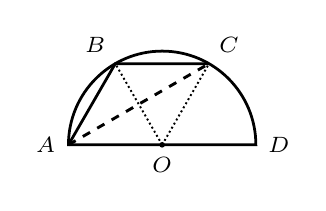
\begin{tikzpicture}[scale=0.68, every node/.style={font=\footnotesize, text=black}]
      \coordinate (O) at (2.0,0.2);
      \fill[white] ($(O)+(0:1.75)$) arc (0:180:1.75) -- cycle;
      \draw[black, line width=1.0pt] ($(O)+(0:1.75)$) arc (0:180:1.75) -- cycle;
      \coordinate (A) at ($(O)+(180:1.75)$);
      \coordinate (B) at ($(O)+(120:1.75)$);
      \coordinate (C) at ($(O)+(60:1.75)$);
      \coordinate (D) at ($(O)+(0:1.75)$);
      \draw[black, line width=1.0pt] (A)--(B)--(C);
      \draw[black, line width=1.05pt, dashed] (A)--(C);
      \draw[black, line width=0.7pt, densely dotted] (O)--(B) (O)--(C);
      \fill[black] (O) circle (1.5pt) node[below=1pt] {$O$};
      \node[left=1pt] at (A) {$A$};
      \node[above left=0.5pt] at (B) {$B$};
      \node[above right=0.5pt] at (C) {$C$};
      \node[right=1pt] at (D) {$D$};
    \end{tikzpicture}
  \end{minipage}
\end{tcolorbox}

% -------------------- ផ្នែកទី២៖ E2 EXPLORE --------------------
\secbar{ផ្នែកទី២ ៖ រុករកតាមខ្នាតពិត \enbf{1:1} និងស្ពានកាំជំនួយត្រីកោណ \enbf{(E2 — Explore)}}{\en{11} នាទី (ពិភាក្សាដៃគូ)}

\begin{tcolorbox}[enhanced, sharp corners, colback=white, colframe=black, boxrule=0.85pt, top=4pt, bottom=4pt, left=6pt, right=6pt]
  \begin{minipage}[c]{9.0cm}
    \centering
    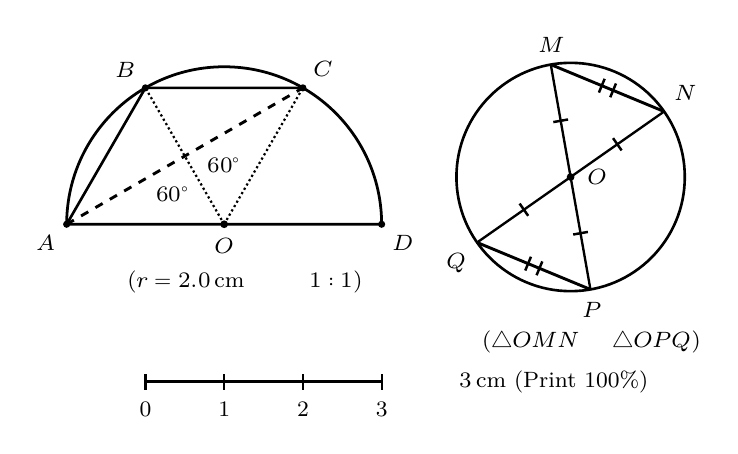
\begin{tikzpicture}[x=1cm, y=1cm, every node/.style={font=\footnotesize, text=black}]
      % រូប ក៖ កន្លះរង្វង់ខ្នាតពិត 1:1 កាំ r = 2.0 cm (AD = 4.0 cm)
      \coordinate (O) at (2.10,1.45);
      \draw[black, line width=1.0pt] ($(O)+(0:2.00)$) arc (0:180:2.00) -- cycle;
      \coordinate (A) at ($(O)+(180:2.00)$);
      \coordinate (B) at ($(O)+(120:2.00)$);
      \coordinate (C) at ($(O)+(60:2.00)$);
      \coordinate (D) at ($(O)+(0:2.00)$);
      \draw[black, line width=0.95pt] (A)--(B)--(C);
      \draw[black, line width=1.05pt, dashed] (A)--(C);
      \draw[black, line width=0.80pt, densely dotted] (O)--(B) (O)--(C);
      \fill[black] (O) circle (1.4pt) node[below=1.5pt] {$O$};
      \fill[black] (A) circle (1.3pt) node[below left=0.5pt] {$A$};
      \fill[black] (B) circle (1.3pt) node[above left=0.5pt] {$B$};
      \fill[black] (C) circle (1.3pt) node[above right=0.5pt] {$C$};
      \fill[black] (D) circle (1.3pt) node[below right=0.5pt] {$D$};
      \node at ($(O)+(150:0.75)$) {$60^\circ$};
      \node at ($(O)+(90:0.75)$) {$60^\circ$};
      \node[anchor=north] at (2.10,0.98) {\textbf{រូប ក} ($r=2.0\unit{cm}$ ខ្នាតពិត $1:1$)};

      % រូប ខ៖ រង្វង់ផ្ចិត O មានត្រីកោណកាំ OAB និង OMN
      \begin{scope}[shift={(4.65,0)}]
        \coordinate (O2) at (1.85,2.05);
        \draw[black, line width=0.95pt] (O2) circle (1.45);
        \coordinate (M1) at ($(O2)+(100:1.45)$);
        \coordinate (N1) at ($(O2)+(35:1.45)$);
        \coordinate (P1) at ($(O2)+(-80:1.45)$);
        \coordinate (Q1) at ($(O2)+(-145:1.45)$);
        \draw[black, line width=0.85pt, tk1] (O2)--(M1);
        \draw[black, line width=0.85pt, tk1] (O2)--(N1);
        \draw[black, line width=0.85pt, tk1] (O2)--(P1);
        \draw[black, line width=0.85pt, tk1] (O2)--(Q1);
        \draw[black, line width=1.05pt, tk2] (M1)--(N1);
        \draw[black, line width=1.05pt, tk2] (P1)--(Q1);
        \fill[black] (O2) circle (1.4pt) node[right=2.5pt] {$O$};
        \node[above=1pt] at (M1) {$M$};
        \node[above right=0.5pt] at (N1) {$N$};
        \node[below=1pt] at (P1) {$P$};
        \node[below left=0.5pt] at (Q1) {$Q$};
        \node[anchor=north] at (1.85,0.22) {\textbf{រូប ខ} ($\tri{OMN}$ និង $\tri{OPQ}$)};
      \end{scope}

      % បន្ទះក្រិតខ្នាតពិត 3 cm (Print 100%)
      \draw[black, line width=0.9pt] (1.10,-0.55) -- (4.10,-0.55);
      \foreach \x/\lbl in {1.10/0, 2.10/1, 3.10/2, 4.10/3} {
        \draw[black, line width=0.8pt] (\x,-0.65) -- (\x,-0.45);
        \node[below=2pt] at (\x,-0.61) {\en{\lbl}};
      }
      \node[right=4pt] at (4.10,-0.55) {\footnotesize ខ្នាតពិត $\en{3\unit{cm}}$ (\en{Print 100\%})};
    \end{tikzpicture}
  \end{minipage}\hfill
  \begin{minipage}[c]{9.2cm}
    \textbf{១. ពិនិត្យរូប ក (អន្ទាក់សមាមាត្រខុស និងអង្កត់ផ្ចិតធំជាងគេ)៖}\\[1.5pt]
    $\bullet$ ប្រើបន្ទាត់ក្រិតវាស់៖ $AB =$ \dotline{1.0cm}$\unit{cm}$, $BC =$ \dotline{1.0cm}$\unit{cm}$ ឯអង្កត់ផ្ចិត $AD =$ \dotline{1.0cm}$\unit{cm}$ ។\\[1.5pt]
    $\bullet$ វាស់ប្រវែងអង្កត់ធ្នូ $AC$ ($\arc{AC}=120^\circ = 2\arc{AB}$)៖ $AC \approx$ \dotline{1.1cm}$\unit{cm}$ ។ តើ $AC = 2AB$ ឬទេ? \chk\ ស្មើ \quad \chk\ មិនស្មើ ($AC < 2AB$)!\\[1.5pt]
    $\bullet$ \textbf{ហេតុផលតាម $\tri{ABC}$៖} $AB + BC$ \dotline{0.8cm} $AC$ (វិសមភាពត្រីកោណ) ។\\[1.5pt]
    $\bullet$ ក្នុង $\tri{OAC}$៖ $OA + OC =$ \dotline{1.0cm}$\unit{cm} = AD > AC \Rightarrow$ អង្កត់ធ្នូវែងបំផុតក្នុងរង្វង់គឺ \dotline{2.2cm} ។\\[3pt]
    \textbf{២. ពិនិត្យរូប ខ (ត្រីកោណកាំ $\tri{OMN}$ និង $\tri{OPQ}$, ទំ.២០១)៖}\\[1.5pt]
    $\bullet$ កាំរង្វង់តែមួយ៖ $OM = ON = OP = OQ =$ \dotline{0.9cm} ។\\[1.5pt]
    $\bullet$ បើធ្នូ $\arc{MN} = \arc{PQ} \Rightarrow \ang{MON} =$ \dotline{1.3cm} $\Rightarrow \tri{OMN}\cg\tri{OPQ}$ តាមករណី \dotline{1.3cm} $\implies MN =$ \dotline{1.1cm} ។\\[1.5pt]
    $\bullet$ ច្រាសមកវិញ បើអង្កត់ធ្នូ $MN = PQ \Rightarrow \tri{OMN}\cg\tri{OPQ}$ តាមករណី \dotline{1.3cm} $\implies \ang{MON} = \ang{POQ} \implies \arc{MN} =$ \dotline{1.1cm} ។
  \end{minipage}
\end{tcolorbox}

% -------------------- ផ្នែកទី៣៖ E3 EXPLAIN --------------------
\secbar{ផ្នែកទី៣ ៖ សំយោគទ្រឹស្ដីបទទាំងបី និងធនាគារហេតុផល \enbf{(E3 — Explain)}}{\en{6} នាទី (ទំ.២០០--២០១)}

\begin{tcolorbox}[enhanced, sharp corners, colback=white, colframe=black, boxrule=0.95pt, top=4pt, bottom=4pt, left=6pt, right=6pt]
  $\bullet$ \textbf{ទ្រឹស្ដីបទទី១៖} \dotline{2.3cm} ជាអង្កត់ធ្នូដែលធំជាងគេនៅក្នុងរង្វង់មួយ ($d = 2r$) ។\\[2pt]
  $\bullet$ \textbf{ទ្រឹស្ដីបទទី២ និងទី៣៖} ក្នុងរង្វង់មួយ (ឬរង្វង់ពីរប៉ុនគ្នា) បើធ្នូប៉ុនគ្នា នោះអង្កត់ធ្នូទាំងពីរ \dotline{1.8cm} ហើយច្រាសមកវិញ បើអង្កត់ធ្នូពីរប៉ុនគ្នា នោះធ្នូដែលសន្ធឹងក្រោមអង្កត់ធ្នូទាំងពីរក៏ \dotline{1.8cm} ដែរ ។\\[2pt]
  $\bullet$ \textbf{វិសមភាពធ្នូតូច (លំហាត់គំរូទី៣ ទំ.២០១)៖} ក្នុងរង្វង់តែមួយ សម្រាប់ធ្នូតូច ($<180^\circ$) បើ $\arc{AB} > \arc{CD}$ នោះអង្កត់ធ្នូ $AB$ \dotline{1.0cm} $CD$ ។\\[3.5pt]
  {\fontsize{8.9pt}{12.5pt}\selectfont
  \begin{tabular}{|L{3.45cm}|L{3.55cm}|L{3.55cm}|L{3.35cm}|L{3.10cm}|}
    \hline
    \cellcolor{headgray}\centering\textbf{\cnum{1} អង្កត់ផ្ចិតធំបំផុត} &
    \cellcolor{headgray}\centering\textbf{\cnum{2} ធ្នូប៉ុន $\Rightarrow$ អង្កត់ធ្នូប៉ុន} &
    \cellcolor{headgray}\centering\textbf{\cnum{3} អង្កត់ធ្នូប៉ុន $\Rightarrow$ ធ្នូប៉ុន} &
    \cellcolor{headgray}\centering\textbf{\cnum{4} វិសមភាពធ្នូតូច} &
    \cellcolor{headgray}\centering\arraybackslash\textbf{\cnum{5} បូក-ដកធ្នូរួម} \\[2pt]
    \hline
    អង្កត់ផ្ចិត $AB = 2r$ ធំជាងគ្រប់អង្កត់ធ្នូ $CD$ ($OC+OD>CD$) &
    $\arc{AB} = \arc{MN} \implies AB = MN$\par (តាម $\tri{OAB}\cg\tri{OMN}$ ជ.ម.ជ) &
    $AB = MN \implies \arc{AB} = \arc{MN}$\par (តាម $\tri{OAB}\cg\tri{OMN}$ ជ.ជ.ជ) &
    បើធ្នូតូច ($<180^\circ$)៖\par $\arc{AB}>\arc{CD} \iff AB>CD$ &
    $\arc{AD}=\arc{CB} \implies$\par $\arc{AD}\pm\arc{CD} = \arc{CB}\pm\arc{CD}$ \\[2pt]
    \hline
  \end{tabular}}
\end{tcolorbox}

\newpage

% ============================================================================
% ទំព័រទី២៖ E4 លំហាត់គំរូបំពេញចន្លោះ + E5 អនុវត្ត & Exit Check + កិច្ចការផ្ទះ
% ============================================================================
\secbar{ផ្នែកទី៤ ៖ លំហាត់គំរូសម្រាយបញ្ជាក់តាមជំហាន \enbf{(E4 — Faded Worked Examples)}}{\en{10} នាទី (ទំ.២០១ និង ២០៤)}

\begin{tcolorbox}[enhanced, sharp corners, colback=white, colframe=black, boxrule=0.90pt, top=4pt, bottom=4pt, left=6pt, right=6pt, after skip=5pt]
  \begin{minipage}[c]{12.7cm}
    \textbf{គំរូទី១ (លំហាត់គំរូទី១ និងទី៣ ទំ.២០១ — ស្រាយវិសមភាពអង្កត់ធ្នូដោយកាំជំនួយ)៖}\\[2pt]
    \textbf{ក) អង្កត់ផ្ចិត $AB$ និងអង្កត់ធ្នូ $CD$ (មិនកាត់តាម $O$)៖} ស្រាយបំភ្លឺថា $AB > CD$ ។\\
    \hspace*{0.3cm}-- ភ្ជាប់កាំជំនួយ $OC$ និង $OD$ ។ ក្នុងត្រីកោណ $\tri{CDO}$ យើងមាន៖ $OC + OD >$ \dotline{1.3cm} $(i)$ ។\\
    \hspace*{0.3cm}-- តែ $OC = OD = r \implies OC + OD = 2r =$ \dotline{1.3cm} $(ii)$ ។ តាម $(i)$ និង $(ii)$ បាន \dotline{1.2cm} $> CD$ ។\\[2pt]
    \textbf{ខ) ធ្នូតូច $\arc{AB} > \arc{CD}$ ក្នុង $C(O,r)$៖} ក្នុង $\tri{AOB}$ និង $\tri{COD}$ មាន $OA=OB=OC=OD=$ \dotline{0.9cm} តែមុំផ្ចិត $\ang{AOB}$ \dotline{0.8cm} $\ang{COD}$ ($\arc{AB}>\arc{CD}$) $\implies$ អង្កត់ធ្នូ $AB$ \dotline{0.8cm} $CD$ (តាម \cnum{4}) ។
  \end{minipage}\hfill
  \begin{minipage}[c]{5.5cm}
    \centering
    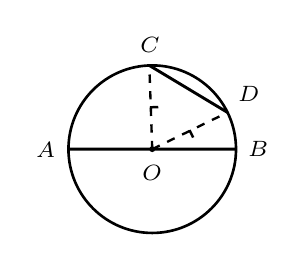
\begin{tikzpicture}[scale=0.76, every node/.style={font=\footnotesize, text=black}]
      \coordinate (O) at (1.7,1.45);
      \draw[black, line width=0.95pt] (O) circle (1.40);
      \coordinate (A) at ($(O)+(180:1.40)$);
      \coordinate (B) at ($(O)+(0:1.40)$);
      \coordinate (C) at ($(O)+(92:1.40)$);
      \coordinate (D) at ($(O)+(26:1.40)$);
      \draw[black, line width=1.05pt] (A)--(B) (C)--(D);
      \draw[black, line width=0.85pt, dashed, tk1] (O)--(C);
      \draw[black, line width=0.85pt, dashed, tk1] (O)--(D);
      \fill[black] (O) circle (1.4pt) node[below=2pt] {$O$};
      \node[left=1pt] at (A) {$A$};
      \node[right=1pt] at (B) {$B$};
      \node[above=1pt] at (C) {$C$};
      \node[above right=0.5pt] at (D) {$D$};
    \end{tikzpicture}
  \end{minipage}
\end{tcolorbox}

\begin{tcolorbox}[enhanced, sharp corners, colback=panelgray, colframe=black, boxrule=0.90pt, top=4pt, bottom=4pt, left=6pt, right=6pt, after skip=5pt]
  \begin{minipage}[c]{12.7cm}
    \textbf{គំរូទី២ (លំហាត់ទី២ ទំ.២០៤ — វិធីដកធ្នូរួមដើម្បីស្រាយថា $AC = BD$)៖}\\
    ក្នុងរង្វង់ $C(O, r)$ ចំណុច $A, C, D, B$ ស្ថិតតាមលំដាប់ដូចរូប ដែលធ្នូ $\arc{AD} = \arc{CB}$ ។ ស្រាយបញ្ជាក់ថាអង្កត់ធ្នូ $AC = BD$ ។\\[2pt]
    $\bullet$ កត់សម្គាល់ធ្នូរួមនៅចន្លោះកណ្ដាលគឺធ្នូ \dotline{1.2cm}៖\\
    \hspace*{0.4cm}$\arc{AD} = \arc{AC} +$ \dotline{1.2cm} \quad និង \quad $\arc{CB} =$ \dotline{1.2cm} $+ \arc{DB}$ ។\\[2pt]
    $\bullet$ ដោយ $\arc{AD} = \arc{CB}$ ដកធ្នូរួម \dotline{1.1cm} ពីអង្គទាំងពីរ (តាមហេតុផល \cnum{5})៖\\
    \hspace*{0.4cm}$\arc{AD} - \arc{CD} = \arc{CB} - \arc{CD} \implies \arc{AC} =$ \dotline{1.3cm} ។\\[2pt]
    $\bullet$ តាមទ្រឹស្ដីបទធ្នូប៉ុនគ្នា (ហេតុផលលេខ \dotline{0.9cm})៖ នាំឱ្យអង្កត់ធ្នូ $AC =$ \dotline{1.3cm} ។
  \end{minipage}\hfill
  \begin{minipage}[c]{5.5cm}
    \centering
    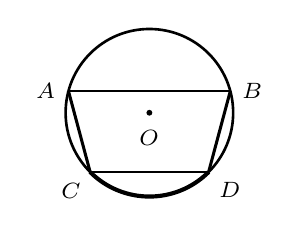
\begin{tikzpicture}[scale=0.76, every node/.style={font=\footnotesize, text=black}]
      \coordinate (O) at (1.7,1.45);
      \draw[black, line width=0.95pt] (O) circle (1.40);
      \coordinate (A) at ($(O)+(165:1.40)$);
      \coordinate (B) at ($(O)+(15:1.40)$);
      \coordinate (C) at ($(O)+(225:1.40)$);
      \coordinate (D) at ($(O)+(315:1.40)$);
      \draw[black, line width=0.85pt] (A)--(B) (C)--(D);
      \draw[black, line width=1.10pt] (A)--(C) (B)--(D);
      \draw[black, line width=1.50pt] (C) arc (225:315:1.40);
      \fill[black] (O) circle (1.4pt) node[below=2.5pt] {$O$};
      \node[left=1pt] at (A) {$A$};
      \node[right=1pt] at (B) {$B$};
      \node[below left=0.5pt] at (C) {$C$};
      \node[below right=0.5pt] at (D) {$D$};
    \end{tikzpicture}
  \end{minipage}
\end{tcolorbox}

% -------------------- ផ្នែកទី៥៖ E5 EVALUATE --------------------
\secbar{ផ្នែកទី៥ ៖ លំហាត់អនុវត្តដោយខ្លួនឯង និងតេស្តវាយតម្លៃរហ័ស \enbf{(E5 — Evaluate)}}{\en{10} នាទី (ទំ.២០៤)}

\noindent
\begin{minipage}[t]{11.3cm}
  \begin{tcolorbox}[enhanced, sharp corners, colback=white, colframe=black, boxrule=0.90pt, top=4pt, bottom=4pt, left=5pt, right=5pt, equal height group=e5c3]
    \textbf{១. អនុវត្តលំហាត់ទី៣ (ទំ.២០៤ — វិធីបូកធ្នូរួម)៖}\\
    គេឱ្យរង្វង់ផ្ចិត $O$ កាំ $r$ ដែលអង្កត់ធ្នូ $AB = CD$ (ចំណុច $A, B, C, D$ ស្ថិតតាមលំដាប់ដូចរូប) ។ ស្រាយបញ្ជាក់ថាធ្នូ $\arc{AC} = \arc{BD}$ ។\\[2pt]
    \begin{minipage}[c]{6.4cm}
      $\bullet$ ដោយអង្កត់ធ្នូ $AB = CD$ (សម្មតិកម្ម)\\
      \hspace*{0.25cm}$\implies$ ធ្នូ $\arc{AB} =$ \dotline{1.3cm} (តាម \dotline{0.9cm}) ។\\[2pt]
      $\bullet$ បូកធ្នូរួម \dotline{1.2cm} ទៅនឹងអង្គទាំងពីរ៖\\
      \hspace*{0.25cm}$\arc{AB} +$ \dotline{1.1cm} $= \arc{CD} +$ \dotline{1.1cm}\\[2pt]
      $\bullet$ ដូចនេះ ធ្នូ $\arc{AC} =$ \dotline{1.4cm} ។
    \end{minipage}\hfill
    \begin{minipage}[c]{4.1cm}
      \centering
      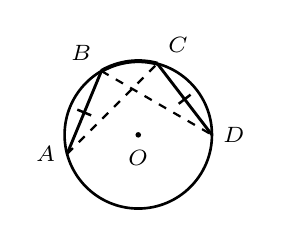
\begin{tikzpicture}[scale=0.72, every node/.style={font=\footnotesize, text=black}]
        \coordinate (O) at (1.5,1.4);
        \draw[black, line width=0.95pt] (O) circle (1.30);
        \coordinate (A) at ($(O)+(195:1.30)$);
        \coordinate (B) at ($(O)+(120:1.30)$);
        \coordinate (C) at ($(O)+(75:1.30)$);
        \coordinate (D) at ($(O)+(0:1.30)$);
        \draw[black, line width=1.05pt, tk1] (A)--(B);
        \draw[black, line width=1.05pt, tk1] (C)--(D);
        \draw[black, line width=0.80pt, dashed] (A)--(C) (B)--(D);
        \draw[black, line width=1.45pt] (C) arc (75:120:1.30);
        \fill[black] (O) circle (1.4pt) node[below=2pt] {$O$};
        \node[left=0.5pt] at (A) {$A$};
        \node[above left=0.5pt] at (B) {$B$};
        \node[above right=0.5pt] at (C) {$C$};
        \node[right=0.5pt] at (D) {$D$};
      \end{tikzpicture}
    \end{minipage}\\[4pt]
    \hrule height 0.4pt\vspace{4pt}
    \textbf{២. ពិនិត្យលក្ខខណ្ឌអង្កត់ធ្នូធំបំផុត៖} រង្វង់ $C(O, 6.5\unit{cm})$ មានអង្កត់ធ្នូវែងបំផុតស្មើនឹង $d = 2r =$ \dotline{1.4cm}$\unit{cm}$ ។ តើអាចគូសអង្កត់ធ្នូប្រវែង $14\unit{cm}$ ក្នុងរង្វង់នេះបានឬទេ? \chk\ បាន \quad \chk\ មិនបាន (ព្រោះ \dotline{2.8cm}) ។
  \end{tcolorbox}
\end{minipage}\hfill
\begin{minipage}[t]{7.4cm}
  \begin{tcolorbox}[enhanced, sharp corners, colback=white, colframe=black, boxrule=0.90pt, top=4pt, bottom=4pt, left=5pt, right=5pt, equal height group=e5c3]
    \textbf{៣. បិទបេសកកម្ម E1 (ស៊ុមបង្អួចកោង)៖}\\
    ពេលធ្នូកើន $2$ ដង ($\arc{AC}=2\arc{AB}$) អង្កត់ធ្នូ $AC$ ធៀបនឹង $2AB$ គឺ៖ $AC$ \dotline{0.9cm} $2AB$ ។\\[4pt]
    \textbf{៤. តេស្តរហ័ស (\en{Exit Check})៖}\\
    ក្នុងរង្វង់ $C(O, 5\unit{cm})$ គេមានធ្នូតូច $\arc{MN} = 70^\circ$ និងធ្នូតូច $\arc{PQ} = 140^\circ$ ។ តើទំនាក់ទំនងណាត្រឹមត្រូវ?\\[3pt]
    \chk\ \textbf{A.} $PQ = 2MN$\\[2.5pt]
    \chk\ \textbf{B.} $PQ = MN$\\[2.5pt]
    \chk\ \textbf{C.} $MN < PQ < 10\unit{cm}$ និង $PQ < 2MN$\\[2.5pt]
    \chk\ \textbf{D.} $PQ = 12\unit{cm}$\\[4pt]
    \textbf{ហេតុផល៖} អង្កត់ផ្ចិតធំបំផុតគឺ $2r =$ \dotline{1.3cm}$\unit{cm}$\\
    ហើយតាមវិសមភាពត្រីកោណ៖ \dotline{3.0cm}
  \end{tcolorbox}
\end{minipage}

% -------------------- ផ្នែកទី៦៖ កិច្ចការផ្ទះ --------------------
\vspace{6pt}
\begin{tcolorbox}[enhanced, sharp corners, colback=panelgray, colframe=black, boxrule=0.95pt, top=4.5pt, bottom=4.5pt, left=6pt, right=6pt]
  \begin{minipage}[c]{14.2cm}
    {\muol\fontsize{9.0pt}{13.5pt}\selectfont ផ្នែកទី៦ ៖ កិច្ចការផ្ទះ និងបណ្ដាំផ្ញើ (សៀវភៅសិក្សាគោល ទំព័រ ២០១ និង ២០៤ — ធ្វើក្នុងសៀវភៅលំហាត់)}\\[2.5pt]
    $\bullet$ \textbf{លំហាត់ទី៥ (ទំ.២០៤)៖} គេឱ្យរង្វង់ $C(O, r)$ ដែលអង្កត់ធ្នូ $AB = CD$ (ចំណុច $A, C, B, D$ ស្ថិតតាមលំដាប់ដូចរូបខាងស្ដាំ) ។ ចូរបង្ហាញថាធ្នូ $\arc{BD} = \arc{AC}$ (ណែនាំ៖ ដកធ្នូរួម $\arc{CB}$ ពី $\arc{AB} = \arc{CD}$) ។\\[2.5pt]
    $\bullet$ \textbf{លំហាត់គំរូទី២ (ទំ.២០១)៖} ក្នុងរង្វង់ផ្ចិត $O$ បើធ្នូ $\arc{MN} = \arc{PQ}$ ចូរសរសេរសម្រាយបញ្ជាក់ថាអង្កត់ធ្នូ $MN = PQ$ តាមត្រីកោណប៉ុនគ្នា និងអានមុនចំណុច \textbf{២.២ លក្ខណៈឆ្លុះនៃរង្វង់} (ទំ.២០២--២០៣) ។
  \end{minipage}\hfill
  \begin{minipage}[c]{4.1cm}
    \centering
    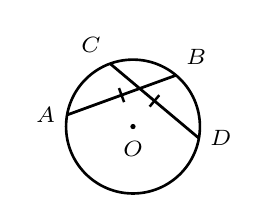
\begin{tikzpicture}[scale=0.68, every node/.style={font=\footnotesize, text=black}]
      \coordinate (O) at (1.5,1.5);
      \draw[black, line width=0.95pt] (O) circle (1.25);
      \coordinate (A) at ($(O)+(170:1.25)$);
      \coordinate (C) at ($(O)+(110:1.25)$);
      \coordinate (B) at ($(O)+(50:1.25)$);
      \coordinate (D) at ($(O)+(-10:1.25)$);
      \draw[black, line width=1.0pt, tk1] (A)--(B);
      \draw[black, line width=1.0pt, tk1] (C)--(D);
      \fill[black] (O) circle (1.4pt) node[below=1.5pt] {$O$};
      \node[left=0.5pt] at (A) {$A$};
      \node[above left=0.5pt] at (C) {$C$};
      \node[above right=0.5pt] at (B) {$B$};
      \node[right=0.5pt] at (D) {$D$};
    \end{tikzpicture}
  \end{minipage}
\end{tcolorbox}

\end{document}
